\section{Reinforcement Learning}
Mit Reinforcement Learning (RL, deutsch: verstärkendes Lernen) werden bestimmte Varianten des maschinellen Lernens bezeichnet. Allgemein lernt beim Reinforcement Learning ein Agent (d.h. ein kontrollierbarer Akteur) eine Policy (deutsch: Strategie), um in einer Umgebung ein Problem zu lösen, das sequentielle Entscheidungen umfasst. Reinforcement Learning ist ein breites Forschungsgebiet. In diesem Grundlagenkapitel werden nur die Grundlagen des Reinforcement Learning beschrieben, die im Rahmen der Projektgruppe relevant sind. Eine Übersicht über weitere Varianten des Reinforcement Learning findet sich z.B. in den Büchern von \citeauthor{FoundationsDeepRL} und \citeauthor{deepRL-2020}.

\subsection{Begriffe des Reinforcement Learning}

\subsubsection{Agent und Umgebung}
\begin{figure}
    \centering
    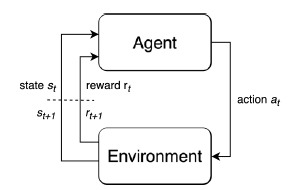
\includegraphics{resources/img/Reinforcement_Learning/RL Control Loop.png}
    \caption{Reinforcement Learning Kontrollfluss \cite{FoundationsDeepRL}}
    \label{fig:rl_control_loop}
\end{figure}

Abbildung \ref{fig:rl_control_loop} stellt den allgemeinen Markov Entscheidungsprozess (MDP) eines Reinforcement Learning Prozesses dar. Der Agent ist in einer Umgebung (Environment) aktiv. In regelmäßigen Schritten sammelt der Agent in der Umgebung Observationen, bestehend aus einem aktuellen Zustand (State) $s_t$, sowie einer Belohnung (Reward) $r_t$, die entweder Null (d.h. keine Belohnung im aktuellen Schritt), oder ein positiver oder negativer Wert sein kann. Die durch den Agent gelernte Policy bildet den State auf eine Aktion $a_t$ ab. Die Aktion wird in der Umgebung ausgeführt. Danach übergibt die Umgebung den neuen State $s_{t+1}$ und die neue Belohnung $r_{t+1}$ an den Agenten \cite{FoundationsDeepRL}.

\subsubsection{Episoden und Trajektorien}
Eine Episode beschreibt die Zeitspanne von der Initialisierung bis zur Terminierung der Umgebung. Eine Trajektorie beschreibt eine Reihe von Tupeln aus State, Aktion und Reward aus den einzelnen Schritten einer Episode. Die Gleichung \ref{eq:trajectory} stellt die mathematische Schreibweise einer Trajektorie dar. Eine Trajektorie enthält durch die Zeitschritte $[0;t]$ indizierte Tupel. Jedes Tupel beinhaltet den Ausgangszustand $s_t$, die ausgeführte Aktion $a_t$ und den dadurch erhaltenen Reward $r_t$ zum Zeitpunkt $t$. Gleichung \ref{eq:return} zeigt die Definition des Returns einer Trajektorie. Der Return ist der summierte Reward der Trajektorie. Auf Basis gesammelter Trajektorien kann der Agent einen Lernvorgang durchführen und die Policy aktualisieren \cite{FoundationsDeepRL}.
\begin{equation}
    \tau = (s_0,a_0,r_0), (s_1,a_1,r_1), \dots, (s_t,a_t,r_t)
    \label{eq:trajectory}
\end{equation}

\begin{equation}
    R(\tau)=\sum_{0}^{t} r_t
    \label{eq:return}
\end{equation}


\subsection{Policy-basierte \& Value-basierte Algorithmen}
Grundsätzlich wird im Reinforcement Learning zwischen Policy-basierten und Value-basierten Algorithmen unterschieden. Diese werden in den folgenden Abschnitten genauer beschrieben. Beide Verfahren haben das grundlegende Ziel, die maximale kumulative Belohnung (Return) zu erhalten.
Es existieren weitere Unterscheidungen zwischen RL-Methoden. Dazu gehört unter anderem die Unterscheidung zwischen modellbasiertem RL und RL ohne Modell. Bei komplexen Umgebungen eignet sich primär das RL ohne Modell, wobei der Agent keine Kenntnisse über Zustandstransitions- und Belohnungsfunktion besitzt, da die Erstellung eines präzisen Modells zu komplex ist. Im Folgenden wird deswegen von modellfreiem RL ausgegangen \cite{deepRL-2020}.

\subsubsection{Value-basierte Algorithmen}\label{sec:value}
Bei Value-basierten Algorithmen wird eine Funktion zum Schätzen der Wertung eines Zustands bzw. eines Zustand-Aktion Tupels gelernt. Aus der Bewertung wird dann eine Policy generiert. Es gibt zwei grundlegende Value-Funktionen.

\begin{equation}
    V^\pi (s)=\mathbb{E}_{s_0=s, \tau \sim \pi} \left[ \sum_{t=0}^T \gamma^t r_t \right]
    \label{eq:v_function}
\end{equation}
\begin{equation}
    Q^\pi (s,a) = \mathbb{E}_{s_0=s,a_0=a,\tau\sim\pi} \left[ \sum_{t=0}^T \gamma^t r_t\right]
    \label{eq:q_function}
\end{equation}
Die V-Funktion (''Value-Function'', siehe Gleichung \ref{eq:v_function}) schätzt den Wert eines Zustandes anhand der diskontierten kumulativen Belohnung einer in diesem Zustand startenden Trajektorie, unter der Annahme, dass der aktuellen Policy gefolgt wird. 
Die Q-Funktion (''Action-Value-Function'', siehe Gleichung \ref{eq:q_function}) schätzt den Wert eines Zustandes unter Durchführung einer Aktion anhand der diskontierten Rewards einer in diesem Zustand startenden Trajektorie, die zuerst die gewählte Aktion durchführt. 
Bei reinen Value-basierten Algorithmen, wird bevorzugt die Action-Value-Funktion $Q^\pi$ verwendet, da sich diese leichter in eine Policy umwandeln lässt \cite{FoundationsDeepRL}. Bei der intuitiven Umwandlung verwendet der Agent als nächste Aktion die Aktion mit dem maximalen Wert der Action-Value-Funktion. Die Berechnung des maximalen Wertes der Action-Value-Funktion ist in kontinuierlichen Aktionsräumen sehr aufwändig, sodass 
Value-basierte Algorithmen sind Proben-effizienter als Policy-based Algorithmen und haben eine niedrigere Varianz. Allerdings kann eine Konvergenz zu einem lokalen Optimum nicht garantiert werden und die Berechnung des maximalen Wertes der Action-Value-Funktion ist bei kontinuierlichen Aktionsräumen sehr aufwändig, sodass Value-basierte Algorithmen bei kontinuierlichen Aktionsräumen schlechter geeignet sind \cite{grokking}.

\subsubsection{Policy-basierte Algorithmen}\label{sec:policy_gradient}
Bei Policy-basierten Algorithmen wählt eine Policy ($\pi$) die nächste Aktion ($a \sim \pi(s)$) aus, die in der Umgebung umgesetzt wird. Diese Policy bzw. ihre Parameter werden direkt durch den Algorithmus gelernt. Es können zwei Arten von Policies verwendet werden. Eine deterministische Policy bildet deterministisch einen Zustand $s$ auf eine Aktion $a$ ab (siehe Gleichung \ref{eq:deterministic_policy}). \cite{FoundationsDeepRL}
\begin{equation}
    \pi(s) = a
    \label{eq:deterministic_policy}
\end{equation}
In der Praxis werden fast ausschließlich stochastische Policies (siehe Gleichung \ref{eq:stochastic_policy}) verwendet.
\begin{equation}
    \pi(a\vert s) = \mathbb{P}_{\pi}\left[ A=a \vert S=s \right]
    \label{eq:stochastic_policy}
\end{equation}
Eine stochastische Policy ordnet für jede Aktion $a$ eine Wahrscheinlichkeit unter Bedingung des Zustands $s$ zu. Aus der entstehenden Verteilung wird dann die Aktion $a$ gesamplet. Policy-basierte Algorithmen lernen die Funktion $\pi$, sodass das Objective maximiert wird.
Policy-basierte Algorithmen können grundsätzlich auf beliebige Aktionstypen angewendet werden, kontinuierliche Aktionsräume sind möglich. Policy-basierte Algorithmen konvergieren garantiert zu einer lokalen, optimalen Policy. Allerdings sind Policy-basierte Algorithmen Proben-ineffizient und haben eine hohe Varianz. \cite{deepRL-2020}

\paragraph{REINFORCE}
Ein Beispiel für einen Policy-basierten Algorithmus ist REINFORCE. Der REINFORCE Algorithmus wird hier verwendet, um die Grundlagen der Policy Optimierung per Policy Gradient einzuführen.
\begin{equation}
    \vartheta \leftarrow \vartheta + \alpha \nabla_\vartheta J(\pi_\vartheta)
    \label{eq:policy_optimization}
\end{equation}
Gleichung \ref{eq:policy_optimization} zeigt die Optimierung einer Policy. Die optimierte Policy entsteht aus der alten Policy, indem eine Anpassung aus Gradient und Objective Funktion ($J(\pi_\vartheta)$) aufaddiert werden.
\begin{equation}
    \nabla_\vartheta J(\pi_\vartheta) = \mathbb{E}_{\tau\sim\pi_\vartheta} \left[ \sum_{t=0}^T R_t(\tau) \nabla_\vartheta log(\pi_\vartheta(a_t\vert s_t))\right]
    ;\; R_t(\tau) = \sum_{t'=t}^T \gamma^{t'-t} r_{t'}
    \label{eq:gradient_objective_function}
\end{equation}
Dabei werden die Parameter $\pi_\vartheta(a_t\vert s_t)$ der Policy angepasst. Ungünstige Aktionen ($R_t(\tau) < 0$) werden weniger wahrscheinlich. Günstige Aktionen ($R_t(\tau) > 0$) werden wahrscheinlicher. \cite{FoundationsDeepRL}

\subsection{Actor-Critic}
Die Actor-Critic Methode ist eine Methode des Reinforcement Learning. Die Actor-Critic Methode kombiniert die Policy-Gradient und die Value-Function Methoden, die in den Abschnitten \ref{sec:policy_gradient} und \ref{sec:value} beschrieben wurden. Der Actor lernt eine Policy (Policy Gradient Methode) und nutzt für das Lernsignal eine durch den Critic gelernte Value-Function (Value-Function Methode). Durch den Critic wird so eine dichte Bewertungsfunktion erzeugt, auch wenn die echten Rewards aus dem Environment nur selten (d.h. an wenigen Zeitpunkten) vorkommen. Der Agent kann dadurch mit gesammelten Teilstücken von Episoden lernen, statt zwingend vollständige Episoden zu benötigen. 

\subsubsection{Advantage-Actor-Critic (A2C)}
Advantage-Actor-Critic ist eine Variante der Actor-Critic Methode, bei der statt einer Value-Funktion eine Advantage-Funktion verwendet wird.
\begin{equation}
    A^\pi(s_t,a_t) = Q^\pi(s_t,a_t) - V^\pi(s_t)
    \label{eq:advantage_function}
\end{equation}
Die Advantage-Funktion bewertet Zustand-Aktion Tupel im Vergleich zum Durchschnitt des Zustandes. Dadurch wird der erreichbare Reward in Relation zur Ausgangssituation gesetzt. Ein kleiner Reward aus einem schlechten Zustand wird somit ebenso gut gewertet, wie ein großer Reward aus einem guten Ausgangszustand. Überdurchschnittliche Aktionen haben also einen positiven Advantage, während unterdurchschnittliche Aktionen einen negativen Advantage haben.
Durch die Verwendung der Advantage-Funktion ändert sich die Formel für den Gradienten. Die Gradienten Formel für die A2C Methode ist in Gleichung \ref{eq:a2c_gradient} dargestellt.
\begin{equation}
    \nabla_\vartheta J(\pi_\vartheta) = \mathbb{E}_t\left[ A_t^\pi (s_t,a_t) \nabla_\vartheta log(\pi_\vartheta(a_t\vert s_t))\right]
    \label{eq:a2c_gradient}
\end{equation}
Für die Berechnung der Advantage-Funktion werden $V^\pi$ und $Q^\pi$ benötigt. Da es sehr ineffizient ist, sowohl $Q^\pi$, als auch $V^\pi$ zu lernen, lernt der Critic nur $V^\pi$ und schätzt auf dieser Grundlage dann $Q^\pi$. Für die Schätzung kann z.B. Generalized-Advantage-Estimation verwendet werden. \cite{FoundationsDeepRL}

\subsubsection{Generalized-Advantage-Estimation (GAE)}
Generalized-Advantage-Estimation (GAE) ist eine Methode, den Advantage anhand einer gelernten $V^\pi$ Funktion zu schätzen. GAE verwendet einen exponentiell gewichteten Durchschnitt von n-step Forward Return Advantages.
\begin{equation}
    A^\pi_{NSTEP} = \left[ (\sum_{i=0}^n \gamma^i r_{t+i}) + \gamma^{n+1} V^\pi (s_{t+n+1}) \right] - V^\pi(s_t)
    \label{eq:nstep}
\end{equation}
Gleichung \ref{eq:nstep} stellt die Berechnung von n-step Forward Return Advantages dar. Dabei werden $n$ Schritte an tatsächlichen Rewards gewertet. Ab dem $n+1$ Schritt wird mit einer gelernten $V^\pi$ Funktion geschätzt. Die tatsächlichen Rewards sorgen für eine hohe Varianz und haben dafür kein Bias, da sie direkt aus der Umgebung gesamplet werden. Die $V^\pi$ Funktion stellt eine Erwartung über alle möglichen Trajektorien dar und weist damit eine geringe Varianz auf. Da die $V^\pi$ Funktion gelernt wurde, entsteht dabei Bias. Mit kleinen Werten für $n$ haben n-step Forward Return Advantages eine geringe Varianz bei hohem Bias, mit großen Werten für $n$ haben n-step Forward Return Advantages eine hohe Varianz bei geringem Bias (Bias-Variance Trade-Off). Allgemeine Aussagen über die Wahl des $n$ Parameters sind schwierig.\\
Generalized Advantage Estimation hebt die explizite Wahl von $n$ aus, indem n-step Forward Return Advantages für verschiedene $n$ Werte gewichtet. kombiniert werden.
\begin{equation}
    A^\pi_{GAE(\gamma,\lambda)} (s_t,a_t) = \sum_{l=0}^\infty (\gamma\lambda)^l \delta_{t+l} ;\; \delta_t = r_t + \gamma V^\pi (s_{t+1}) - V^\pi(s_t)
    \label{eq:gae}
\end{equation}
Die allgemeine Formel für GAE ist in Gleichung \ref{eq:gae} abgebildet. Die Gewichtung wird durch die Decay-Rate $\gamma \in [0;1]$ und den Discount-Factor $\lambda \in [0;1]$ parametrisiert.
In der Praxis wird statt der unendlichen Summe eine Summe bis zum Ende der verfügbaren Trajektorie verwendet. \cite{gaePaper}


\subsection{Proximal Policy Optimization (PPO)}
Proximal Policy Optimization (PPO) ist ein Reinforcement Learning Algorithmus, der die Actor-Critic Methode umsetzt.

\subsubsection{Performance Collapse}
Ein Problem von Reinforcement Learning Algorithmen ist der Performance Collapse (Leistungseinbruch). Performance Collapse bedeutet, dass die Returns der Umgebung im Lernvorgang plötzlich einbrechen, da z.B. die Policy über ein lokales Optimum heraus optimiert wurde und der Gradient nun zu einem schlechteren lokalen Optimum konvergiert. Die Ursache für das Problem ist der indirekte Ansatz der Policies. Ein RL Algorithmus manipuliert die Parameter der Policy, um diese zu verändern. Kleine Veränderungen in den Parametern können dabei große Veränderungen in der Policy auslösen \cite{FoundationsDeepRL}. Da die Trainingsdaten mit der aktuellen Policy gesammelt werden, kann ein Performance Collapse dazu führen, dass die kollabierte Policy sich nicht mehr erholt. 

% \paragraph{Surrogate Objective}
% Ein Lösungsansatz für das Performance Collapse Problem ist das Einschränken der Größe einzelner Lernschritte. Dieser Ansatz wurde mit dem Trust Region Policy Optimization Algorithmus (TRPO) (\ref{}) eingeführt, auf dem PPO aufbaut. 
% \begin{equation}
%     J(\pi') - J(\pi) = \mathbb{E}_{\tau \sim \pi} \left[ \sum_{t=0}^T \gamma^t A^\pi(s_t,a_t) \frac{\pi'(a_t\vert s_t)}{\pi(a_t\vert s_t)} \right] = J_\pi^{CPI}(\pi')
%     \label{eq:surrogate_objective}
% \end{equation}
% Gleichung \ref{eq:surrogate_objective} zeigt das sogenannte Surrogate Objective $J_\pi^{CPI}$, das von TRPO verwendet wird um die 

\subsubsection{Clipping}
Es gibt zwei theoretische Varianten des PPO Algorithmus. Die erste Variante baut direkt auf dem Trust Region Policy Optimization Algorithmus (TRPO) \cite{trpoPaper} auf und verwendet eine adaptive KL Penalty, um die Schrittgröße einzuschränken. Diese wird hier nicht weiter beschrieben, da in der Praxis nur die zweite Variante von PPO verwendet wird, weil diese in Tests bessere Ergebnisse erzielt und leichter zu implementieren ist.
Die zweite PPO Variante nutzt ein Clipped Surrogate Objective.
\begin{equation}
    J^{CLIP}(\vartheta) = \mathbb{E}_t\left[ \min(r_t(\vartheta)A_t,clip(r_t(\vartheta),1-\epsilon,1+\epsilon)A_t \right]
    \label{eq:clipped_surrogate_objective}
\end{equation}
Die Gleichung \ref{eq:clipped_surrogate_objective} zeigt das Clipped Surrogate Objective, das vom PPO Algorithmus maximiert wird. Eine Veränderung außerhalb des Bereichs $[1-\epsilon; 1+\epsilon]$ wird dabei geclippt (abgeschnitten) und somit die Schrittgröße eingeschränkt.
\begin{equation}
    J^{CLIP+VF+S}(\vartheta) = \mathbb{E}_t \left[ J_t^{CLIP} - c_1L_t^{VF} + c_2S[\pi_\vartheta(s_t)] \right]
    \label{eq:ppo_objective}
\end{equation}
Die für die Clipped Surrogate Objective Variante des PPO Algorithmus verwendete Loss Funktion wird in Gleichung \ref{eq:ppo_objective} gezeigt. Zusätzlich zum Clipped Surrogate Objective wird der Loss der Value-Funktion und ein Entropie Bonus zur Steigerung der Exploration berechnet. In der Praxis wird das Objective negiert, damit Gradient Descent statt Gradient Ascent durchgeführt werden kann. \cite{PPOPaper}

\paragraph{Algorithmus}

\begin{algorithm}
\begin{lstlisting}[mathescape=true, numbers=left]
for episode=0...MAX do
    for actor=1...N do
        Sample Trajectory for T time steps with $\pi_{\vartheta_{old}}$
        Compute advantage estimates $A_1,\dots,A_T$ with $\pi_{\vartheta_{old}}$
    Collect all states in batch of size N*T
    for epoch=1...K do
        for minibatch of size m in batch do
            Optimize Clipped Surrogate Objective L w.r.t. $\vartheta$
    $\vartheta_{old} = \vartheta$
\end{lstlisting}
\caption{PPO Pseudocode Algorithmus \cite{FoundationsDeepRL}}
\label{alg:ppo}
\end{algorithm}

Algorithmus \ref{alg:ppo} zeigt den Pseudocode des PPO Algorithmus. Für jede Episode wird zuerst pro Actor eine Trajektorie in der Umgebung gesamplet. Dabei werden die Aktionen jeweils durch die aktuelle Policy $\pi_{\vartheta_{old}}$ bestimmt. Für diese Trajektorie werden die zugehörigen Advantages mit GAE berechnet. 
Mit den gesampleten Trajektorien wird die Policy in Epochen trainiert. In jeder Epoche werden Minibatches aus dem gesampleten Batch generiert. Mit den Daten der Minibatches wird das Clipped Surrogate Objective optimiert.